\subsubsection{Gang of Four}\label{sec:gang4}


The design patterns introduced by the Gang of Four will be described briefly, bearing in mind their likely relevance to project \nep.
It is notable that, in the light of the decades of software engineering practice that have followed the publication of \cite{gammahelmjohnsonvlissides}, developments in object-oriented languages themselves have incorporated some of the patterns directly.
Note that the Wikipedia articles on these patterns are largely of good quality and provide also UML representations and (polyglot) code examples.
Note additionally that the Wikipedia article on {\it Software design pattern} \cite{softwarepatternwiki} contains patterns in addition to those in the Go4 text, particularly a fourth category, concerning concurrency patterns, which would seem quintessential to our case.

\subsubsection*{Creational Design Patterns}

These are associated with object creation.

{\it Abstract factory} - this provides an interface for creating {\it families} of related objects without specifying their concrete class.
Derived factory classes create, for example, documents with a style (fonts etc.) common to the concrete factory, the documents being represented by derived types eg.\ fancyLetter, businessLetter, ... , businessReport.  The client only knows about the abstract document types (letter, report ...) and the abstract factory, the concrete choice of which determines the style of documents received by the client.

{\it Builder} - this separates the construction of a complex object from the representation of that object.
Instead of having classes call the object's constructor, they call a separate Builder method that constructs the objects.
Altering this Builder means the object can be constructed differently without having to change the object; also, selecting a different Builder means that the type of object created can be changed.

{\it Factory method} - this decouples the construction of objects from the objects themselves, allowing the creation of objects whose concrete type is not determined at compile time.

{\it Prototype} - this creates objects by cloning an existing object.
The point is that a Clone() method may be called on an object of unspecified concrete type - this is similar to the aim of the Factory method above.

{\it Singleton} - this restricts a class to having a solitary instance (or none at all).
Constructors are hidden by making them private and the sole instance is accessed via a GetInstance() method, which provides global access and can be used to provide lazy initialization - creating the singleton only when it is required.

\subsubsection*{Structural Design Patterns}

These are to do with composition, inheritance etc.; some of them seem very straightforward.
Others appear directly relevant for \nep \ : these examples are presented first and are illustrated with the appropriate UML diagram (all of which were created using the free graphing software {\it yEd} \cite{yedwebsite}).

{\it Adapter} - sometimes known as a wrapper, an Adapter is simply an object that translates between otherwise-incompatible interfaces, thus allowing objects to co-operate without changes to their interfaces.
Arguably one goal of good interface design is to avoid the need for this pattern; however, and with no pejorative intended, since pre-written third-party code may be used in \nep \ , it may well be necessary to use Adapters.  It is also of note that modern-day unified APIs for heterogeneous computing are, fundamentally, implementations of this pattern (eg.\ a SYCL plug-in acts basically as an Adapter for CUDA in order to harness NVidia GPUs). 

\begin{figure}
\begin{centering}
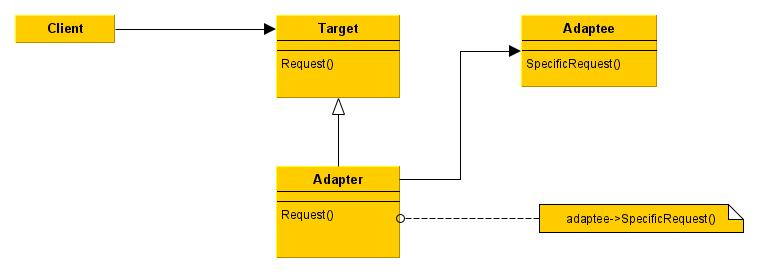
\includegraphics[width=12cm]{../png/adapter.jpg}
\end{centering}
\caption{Class diagram for the (object) Adapter pattern (there is also a very similar class Adapter version).\label{fig:adapter}}
\end{figure}

{\it Composite} - this means the provision of a unified interface for part and whole; eg.\ resizing a collection of shapes is simply resizing each shape.
Branches forward request to leaves (shapes in this case); another example is printing a collection of graphics objects (which boils down to printing each object).  This is certainly relevant to a graph-based approach and indeed it is used in the {\it Arcos} framework.

\begin{figure}
\begin{centering}
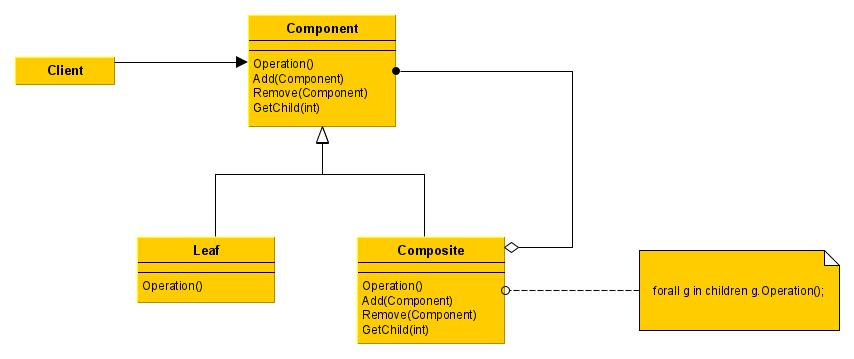
\includegraphics[width=12cm]{../png/composite.jpg}
\end{centering}
\caption{Class diagram for the Composite pattern.\label{fig:composite}}
\end{figure}

{\it Facade} - this means the provision of a simplified API that delegates to interfaces of subsystems; it can thus be used to provide a greater or lesser degree of automation and it also means that all controls of a set of related subsystems are located conveniently in one place (perhaps a reasonable analogy is having all the controls needed to drive a car in front of the driver).
This paradigm seems central to making software easy to use and understand and thus seems to be of great import.

\begin{figure}
\begin{centering}
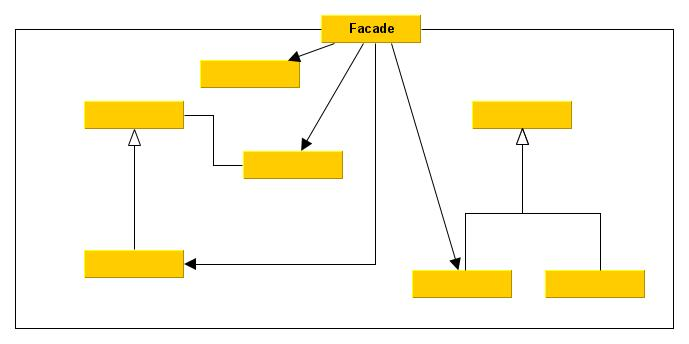
\includegraphics[width=12cm]{../png/facade.jpg}
\end{centering}
\caption{Class diagram for the Facade pattern.\label{fig:facade}}
\end{figure}

{\it Proxy} - this means a class functioning as a stand-in for something else and sharing the same interface.
Clients cannot necessarily distinguish between the object and its proxy, but the latter could provide, for example, additional checking for reasonableness of inputs, or security checking, or implement load-on-demand of data.
The idea of loading large data objects only when explicitly required is of great utility, particularly in a parallel computing scenario.

\begin{figure}
\begin{centering}
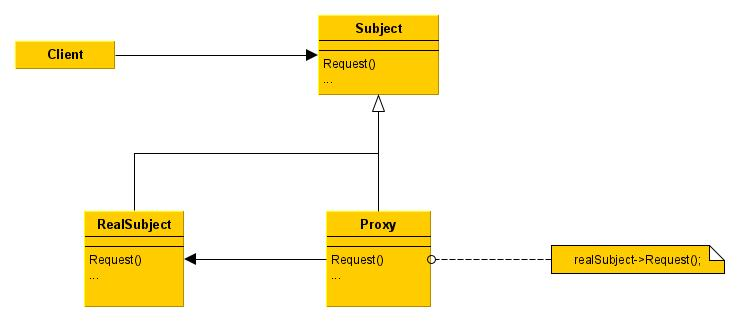
\includegraphics[width=12cm]{../png/proxy.jpg}
\end{centering}
\caption{Class diagram for the Proxy pattern.\label{fig:proxy}}
\end{figure}

The remaining structural patterns were judged to be of lesser interest for project \nep \ .

{\it Bridge} - this decouples abstraction from interface; the bridge object associates an abstraction (=interface) with its implementation at run-time.
This seems very similar to virtual functions (run-time polymorphism).
It seems that the goal of this pattern can be accomplished with virtual methods.

{\it Decorator} - this means adding functionality to a particular object without affecting the behaviour of other objects of same class.
The Decorator object just wraps the class and either overrides or forwards requests.
The constructor of the Decorator has a reference to the decorated object as its argument.
This seems a rather {\it ad hoc} way to add functionality {\it ex post facto}. 

{\it Flyweight} - this seems to mean the sharing of data between similar objects to save memory, eg.\ not storing all the letters in a document but rather storing each letter once (ie.\ an alphabet!) and then the document is represented by a collection of references to these.
It is clearly useful when objects occur in large numbers (again, letters in a document).
The jargon is that intrinsic data (eg.\ the glyph for each letter) can be shared; extrinsic data cannot.
Note that, perhaps counter-intuitively, Flyweight objects are generally big (`bulky data'); they are addressed by references that store only the extrinsic data (in the document example, this would be the positions of the letters).
The reasoning behind the name seems to be that the amount of data stored would be much larger
or heavier if the object was fully described at each occurrence. Thus in the example of letters
in a document, if each were stored with its case, font type and size, this would use up far more
store than stating the font at the beginning.

\subsubsection*{Behavioural Design Patterns}

Three of these patterns were judged to be of somewhat greater interest:

{\it Command} - this means having an encapsulated Command object (constituted by all the information needed to perform an action).  This can be used in scripting, macro recording, multi-level undo, parallel processing, thread pools ... this is, potentially, a key part of overall program coordination.

\begin{figure}
\begin{centering}
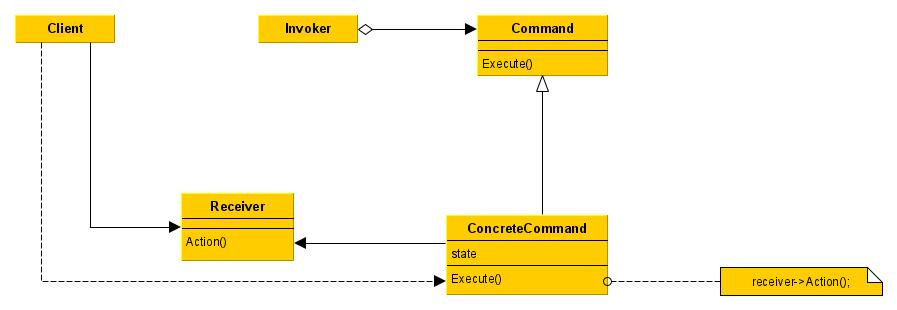
\includegraphics[width=12cm]{../png/command.jpg}
\end{centering}
\caption{Class diagram for the Command pattern.\label{fig:command}}
\end{figure}

{\it Observer} - the subject (an object) maintains a list of dependants and notifies them automatically of any state changes.
It enables commands to be broadcast to all relevant parties (one might draw the analogy of hormones in animal bodies, or pheromones in eusocial insect colonies).  This would appear to be a powerful tool for program coordination.
Also, it is very useful in GUIs for making sure all aspects of the interface are updated to reflect changes in user inputs or data.

\begin{figure}
\begin{centering}
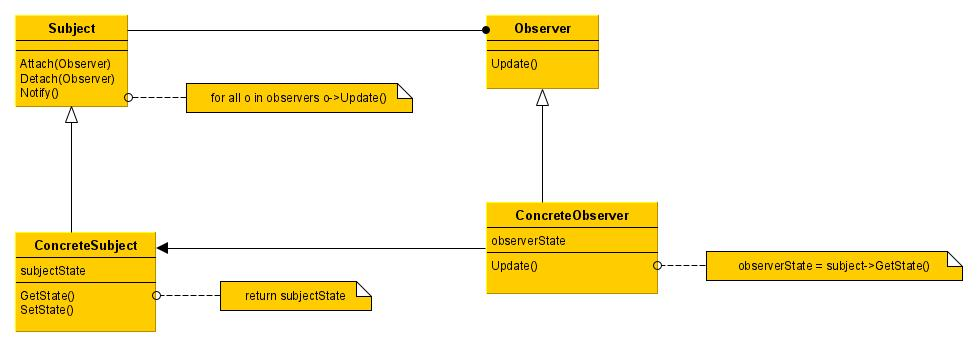
\includegraphics[width=12cm]{../png/observer.jpg}
\end{centering}
\caption{Class diagram for the Observer pattern.\label{fig:observer}}
\end{figure}

{\it Strategy} - also known as Policy, this pattern enables the selection of an algorithm at run-time, perhaps through the use of a run-time-assigned function pointer.
It allows the algorithm to vary independently from the clients that use it.
This can be very useful for the dynamical coupling of objects of arbitrary type.

\begin{figure}
\begin{centering}
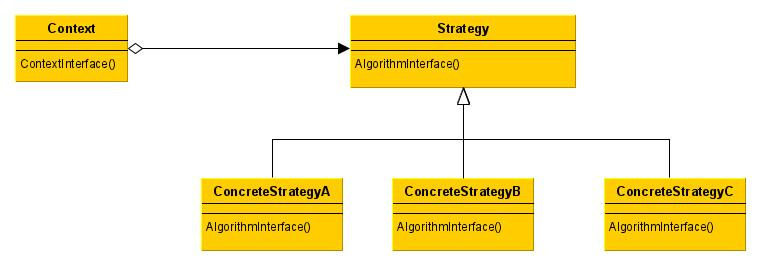
\includegraphics[width=12cm]{../png/strategy.jpg}
\end{centering}
\caption{Class diagram for the Strategy pattern.\label{fig:strategy}}
\end{figure}

In the interest of completeness, the remaining behavioural patterns follow.

{\it Chain of Responsibility} - in this pattern, a command object emitted by a source is passed along a (possibly branching) chain of potential processing objects, representing a dynamical `if ... else if ... else if ...'; it seems to require a nerve-like chain to conduct the command.
The removal of close coupling appeals, though the Observer pattern appears more flexible as it removes the need for the chain / tree of command.

{\it Interpreter} - this means basically providing a domain-specific language with its own grammar, rather than hard-coding each individual command.
Example: instead of writing DO\_A\_WITH\_B() the grammar is Execute(DO A WITH B).
This is useful because grammar can make the driver syntax much cleaner.

{\it Iterator} - this means the ability to access elements of an aggregate object without exposing the underlying representation.
Note that one criticism of Go4 is that it listed features that ought to have been part of C++ and now it seems that some of the patterns have been incorporated in the language - I believe the STL Iterator implements this pattern.
This pattern would appear to be already present in C++, in a sense; otherwise, it seems simply to mean that the API of an aggregate object should hide the implementation, which is something of a given.

{\it Mediator} - this is intended to reduce close coupling between objects, as they communicate via the mediator, rather than directly.
Again it is nice that close coupling is reduced but this scheme does introduce the central control object (mediator), which may not always be desirable.
A single mediator object may have unwanted consequences in a massively-parallel environment (though one can imagine hierarchies of mediators).

{\it Memento} - this involves the provision of the ability to restore an object to a past state (eg.\ for rollback undo).
It seems that an object must store a copy of its past self and some additional information about how to get from that copy to the present version (mathematically, this seems like the Markov property).

{\it State} - means allowing an object to alter its behaviour when its internal state changes. 	One defines State objects (and derives special cases of States), then classes delegate state-specific behaviour to their State object.  The advantages of this pattern are presently unclear; it seems there are also cases when one wants objects {\it not} to have internal state data at all ...

{\it Template method} - here, the skeleton of a method is located in a superclass; the `template' that is never overridden, this contains invariant parts of the algorithm.
Its components {\it are} overridden; for example, one might have a computer game with invariant structure Initialize(), Startplay(), Endplay(), all of which are overrides.  This might be quite useful for different physics solvers; it is obviously logical to have only one copy of common code.

{\it Visitor} - this means adding new virtual functions to a family of classes without modifying the classes or defining a new operation for a class without changing the class: one calls a Visitor method on an object and the Visitor does something to the object.
It is useful for performing an operation on a wide variety of classes without having to put a new method in each class.
It is obviously good `economics' to have only one copy of common code.

\subsubsection{Post-Go4 Patterns}\label{sec:postgang4}

The Wikipedia page on {\it software design pattern} \cite{softwarepatternwiki} outlines a further 16 {\it concurrency patterns}, defining them as {\it`those types of design patterns that deal with the multi-threaded programming paradigm'}.  
Five of these are to be found in the text {\it Pattern-Oriented Software Architecture Vol.2: Patterns for Concurrent and Networked Objects} by Schmidt, Stal, Rohnert and Buschmann (another gang of four) \cite{schmidtstalrohnertbuschmann}.  
Given the lie of the current high-performance computing landscape, these would seem of particular relevance to \nep \  and so, a brief outline of each is given here.

{\it Active object} - method execution is here decoupled from method invocation in order to avoid race conditions on an object's data (or indeed the need	 to write additional code to synchronize such cases).  
Instead of object methods acting directly on the object, the work is delegated to a task scheduler: the upshot is that only one thread may ever modify the internal state of an object.  
The pattern uses {\it asynchronous method invocation}, itself a further pattern.

{\it Balking} - this means that an action is performed on an object solely if that object is in a particular state.  
There is some debate as to the validity of this as a pattern and one might argue that an API should not support requests that are `invalid' in the sense of being inconsistent with the internal state of the object.  
Regardless, the pattern can be used to ensure that a worker object only accepts new jobs if it is not in a `busy' state, for example.

{\it Binding properties} - though the Wikipedia article is somewhat unclear, it seems that this means having multiple observers enforce synchrony (or some other consistency) of the properties of some other object; it would give a way of automatically enforcing mutual consistency of properties of different objects.

{\it Compute kernel} - this is a routine compiled for execution on an accelerator, for example a shader routine of a GPU that is called by the main program.  
The kernel corresponds roughly to the `inner loop' ie.\ the actual work.  
SIMD intrinsics would seem an example of this paradigm also.  
More succinctly: the same computation, many times in parallel.

{\it Double-checked locking} - this seems to mean doing a check on a lock using a criterion (known as the `lock hint') before explicitly acquiring the lock.  
Locking only proceeds in the lock hint indicates that locking is required.  
It is a method of reducing overhead by doing a quick (and possibly dirty - the Wikipedia article cautions that the pattern can be unsafe on certain combinations of hardware / software / language) check before proceeding with an operation.

{\it Event-based asynchronous} - this seems intended to address problems with the {\it asynchronous method invocation} (referred to above, in {\it Active object}), also known as simply the {\it asynchronous} pattern, which means that a long-running method returns immediately a `working ...' response and notifies the caller on later completion of the work.  
One says the caller is not `blocked' (that is the meaning of asynchronous; the Wikipedia article \cite{softwarepatternwiki} does not detail the precise meaning of {\it event-based asynchronous}).

{\it Guarded suspension} - seemingly an alternative to the {\it balking} pattern, this pattern prevents acquisition of a lock until a precondition is satisfied (it is a way of making a program wait before doing something, for example waiting for an queue to contain an object before attempting to operate on an object in the queue).

{\it Join} - {\it join-patterns} refer to the high-level (as opposes the nitty-gritty of threads and locks) practice of making programs work in parallel by {\it message passing}, enabling scalability.  
The article linked from \cite{softwarepatternwiki} contains much detail on {\it join-calculus}.

{\it Lock} - this is a foundation of multi-threaded programming: one thread puts a `lock' on a resource, preventing other threads from accessing or modifying that until the lock is released by the subject thread.

{\it Messaging design pattern (MDP)} - this describes how a communications protocol works, for example request-response (like HTTP) or one-way (like UDP), or request with optional response. 

{\it Monitor object} - this seems to refer to using mutexes (which can be implemented simply as the acquisition of a lock) in order to permit access to the methods of an object on a serial basis only.  
Succinctly: an object whose methods are subject to mutual exclusion.

{\it Reactor} - this is {\it`an object providing an asynchronous interface to resources that must be handled synchronously'} (Wikipedia).  
The object (or {\it service handler}) is said to {\it demultiplex} incoming requests and pass them on in a synchronous manner.

{\it Read-write lock} - this means the provision of concurrent read but serial write access.

{\it Scheduler} - this means the means by which work is doled out to threads; clearly the issue of load-balancing and overall rate-limiting steps raise their heads here.  
Aside - this concept also allowed multi-tasking back in the days of single-processor architectures.

{\it Thread pool} - this refers to a set of threads that are available to be assigned work; the threads may be organized in some way eg.\ as a queue.

{\it Thread-specific storage} - {\it`Static or `global' memory local to a thread.'} (\cite{softwarepatternwiki}).


